
\chapter{开发过程}

\section{Bug修复以及简单功能的完善}

\begin{itemize}
  \item \textbf{Bug修复:}
  \begin{itemize}
      \item 修复总价浮点数精度 bug;
      \item 修复页面显示不全的 bug。
  \end{itemize}
  \item \textbf{功能完善:}
  \begin{itemize}
      \item 手机号的正则表达式检验;
      \item 强密码检验。
  \end{itemize}
\end{itemize}


\section{饿了吧V2.0版本的创新点}
% 插入创新点信息

\subsection{实现前端 Vue2 到 Vue3 的升级}

\subsection{实现“我的”页面}

\begin{figure}[H]
\centering
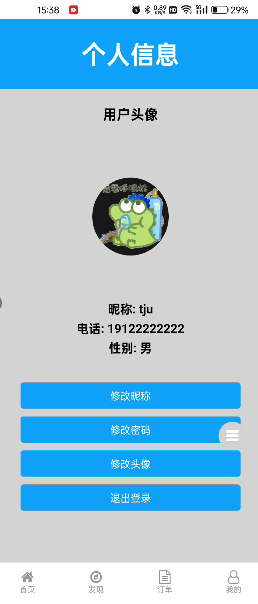
\includegraphics[width=0.4\textwidth]{Picture5}
\caption{实现“我的”页面}\label{fig:xml}
\end{figure}


\subsection{实现修改昵称,修改头像,修改密码功能}

\begin{figure}[H]
  \centering
  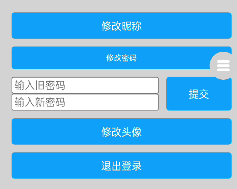
\includegraphics[width=0.4\textwidth]{Pictur6}
  \caption{实现修改昵称,修改头像,修改密码功能}\label{fig:xml}
  \end{figure}

\subsection{实现收藏功能:收藏商家,取消收藏,收藏列表}

\begin{figure}[H]
  \centering
  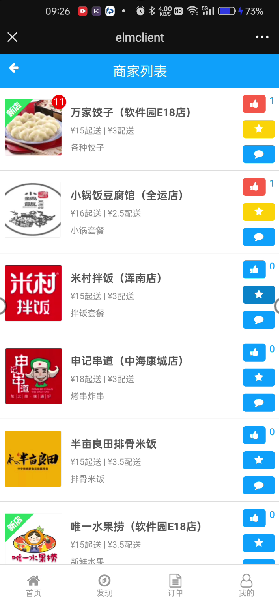
\includegraphics[width=0.4\textwidth]{Picture7}
  \caption{实现收藏功能:收藏商家,取消收藏,收藏列表}\label{fig:xml}
  \end{figure}

\subsection{实现点赞功能:点赞,取消点赞,展示商家总点赞量}

\begin{figure}[H]
  \centering
  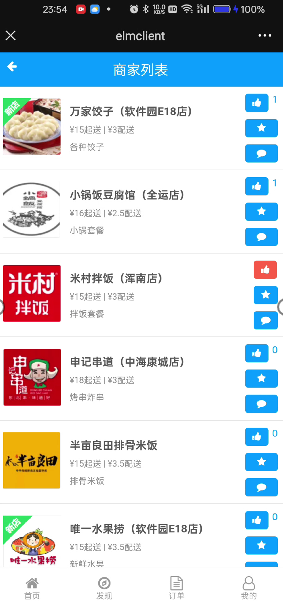
\includegraphics[width=0.4\textwidth]{Picture8}
  \caption{实现点赞功能:点赞,取消点赞,展示商家总点赞量}\label{fig:xml}
  \end{figure}

\subsection{实现评论功能:新增评论,展示评论列表,删除评论}

\begin{figure}[H]
  \centering
  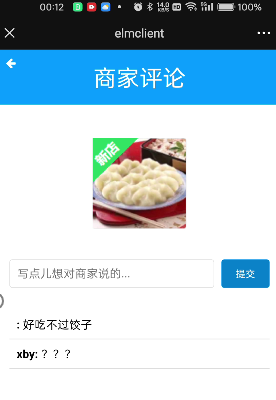
\includegraphics[width=0.4\textwidth]{Pictur9}
  \caption{实现评论功能:新增评论,展示评论列表,删除评论}\label{fig:xml}
  \end{figure}

\subsection{实现搜索功能:模糊匹配,可以搜索商家或商品}

\begin{figure}[H]
  \centering
  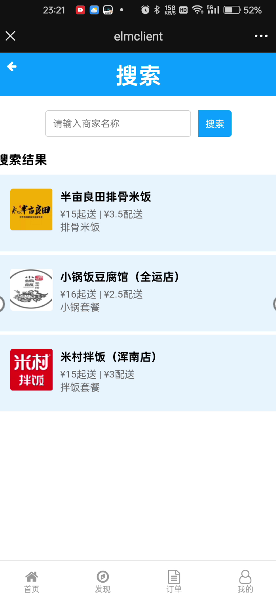
\includegraphics[width=0.4\textwidth]{Picture10}
  \caption{实现搜索功能:模糊匹配,可以搜索商家或商品}\label{fig:xml}
  \end{figure}

\subsection{实现历史记录功能:搜索的时候展示搜索历史}

\begin{figure}[H]
  \centering
  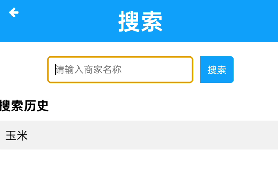
\includegraphics[width=1\textwidth]{Picture11}
  \caption{实现历史记录功能:搜索的时候展示搜索历史}\label{fig:xml}
  \end{figure}

\subsection{实现商家账号注册,登录,上架商品,修改商家个人信息}

\begin{figure}[H]
  \centering
  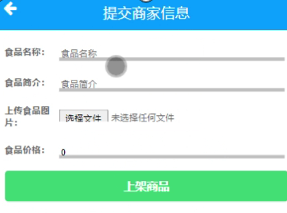
\includegraphics[width=1\textwidth]{Picture12}
  \caption{实现商家账号注册,登录,上架商品,修改商家个人信息}\label{fig:xml}
  \end{figure}

  \subsection{集成文心一言接口,充当智能客服,方便用户对食品的咨询}

  \begin{figure}[H]
  \centering
  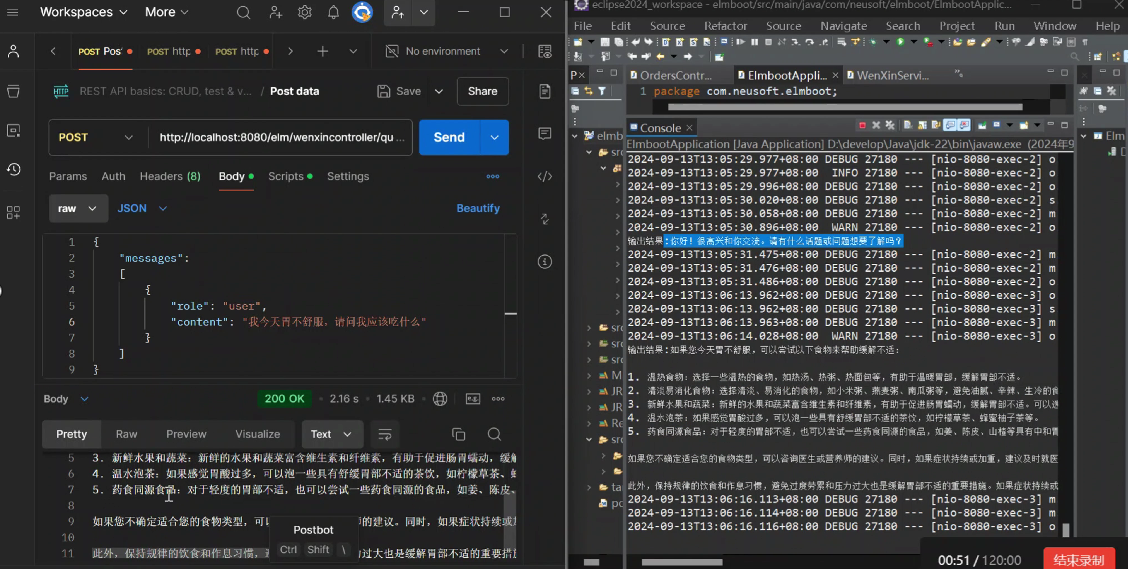
\includegraphics[width=1\textwidth]{Picture13}
  \caption{集成文心一言接口,充当智能客服,方便用户对食品的咨询}\label{fig:xml}
  \end{figure}


\section{部署成果}

\subsection{在腾讯云服务器上部署:前端,后端,数据库}

\begin{figure}[H]
  \centering
  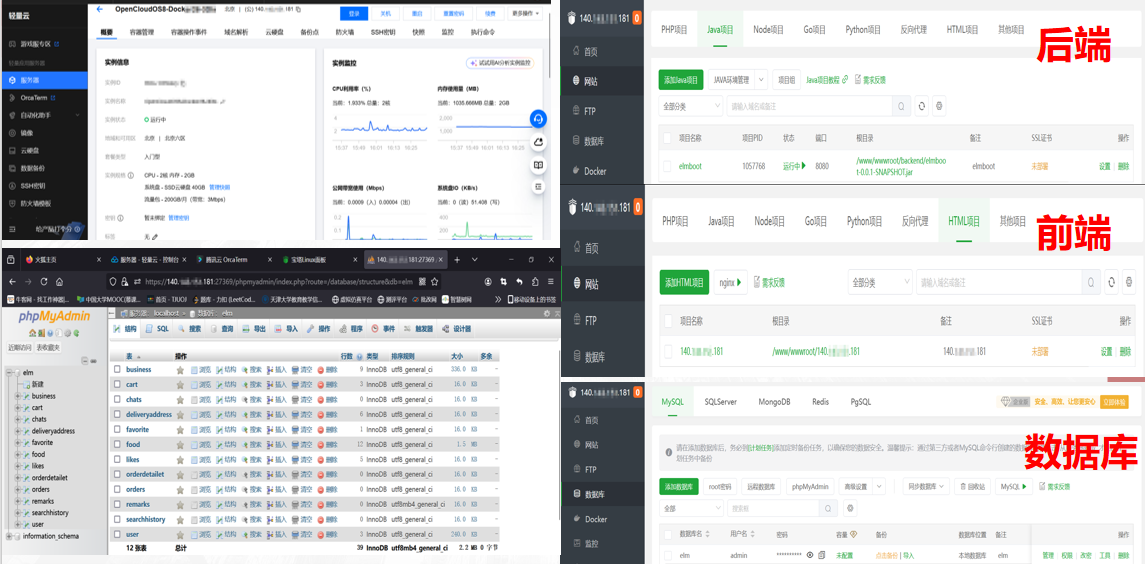
\includegraphics[width=1\textwidth]{Picture14}
  \caption{在腾讯云服务器上部署:前端,后端,数据库}\label{fig:xml}
  \end{figure}
\subsection{创建手机 APK}

\begin{figure}[H]
  \centering
  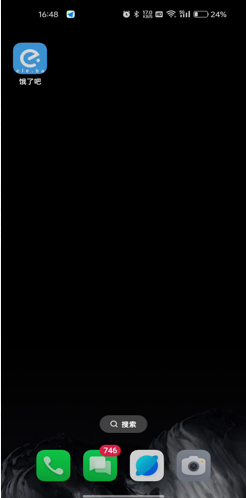
\includegraphics[width=0.4\textwidth]{Picture15}
  \caption{创建手机 APK}\label{fig:xml}
  \end{figure}

